\chapter{Cinética de eletrodo e eletroanálise}\label{ch:b3:electrode-kinetics}

Uma gota de sangue em uma tira de plástico, cinco segundos, um número: o
glicosímetro que milhões de pessoas usam várias vezes por dia é uma célula
eletroquímica, e o que ele mede não é uma tensão, mas uma corrente. Uma \omterm{def:b3:complex-kinetics:enzyme}{enzima}
oxida a glicose, um complexo de ferro dissolvido leva os elétrons até um eletrodo
de carbono, e a corrente que passa é fixada pela velocidade com que esse complexo
se difunde até o eletrodo, logo por sua concentração. Este capítulo explica por
que os elétrons atravessam uma interface depressa ou devagar (a \omterm{thm:b3:electrode-kinetics:butler-volmer}{equação de
Butler--Volmer}), como o transporte de massa limita a corrente e como a
\omterm{def:b3:electrode-kinetics:cv}{voltametria cíclica} e os outros métodos eletroanalíticos transformam correntes
em concentrações, constantes de velocidade e mecanismos.

\begin{recall}
O volume do 1.º ano definiu o potencial de eletrodo, o potencial padrão, a
equação de Nernst, os eletrodos de referência e as meias-pilhas. O volume do
2.º ano introduziu as curvas corrente--potencial com suas correntes anódica e
catódica, os eletrodos de trabalho e os contraeletrodos, as sobretensões, os
sistemas rápidos e lentos, a camada de difusão e a corrente limite; os
coeficientes de atividade e a força iônica; as curvas de calibração, o método da
adição padrão e o limite de detecção. O \cref{ch:b3:rate-theories} deu a \omterm{def:b3:rate-theories:tst}{teoria
do estado de transição}. Da física: as leis de Fick da difusão, a equação de
Poisson e os capacitores.
\end{recall}

\begin{omfigure}
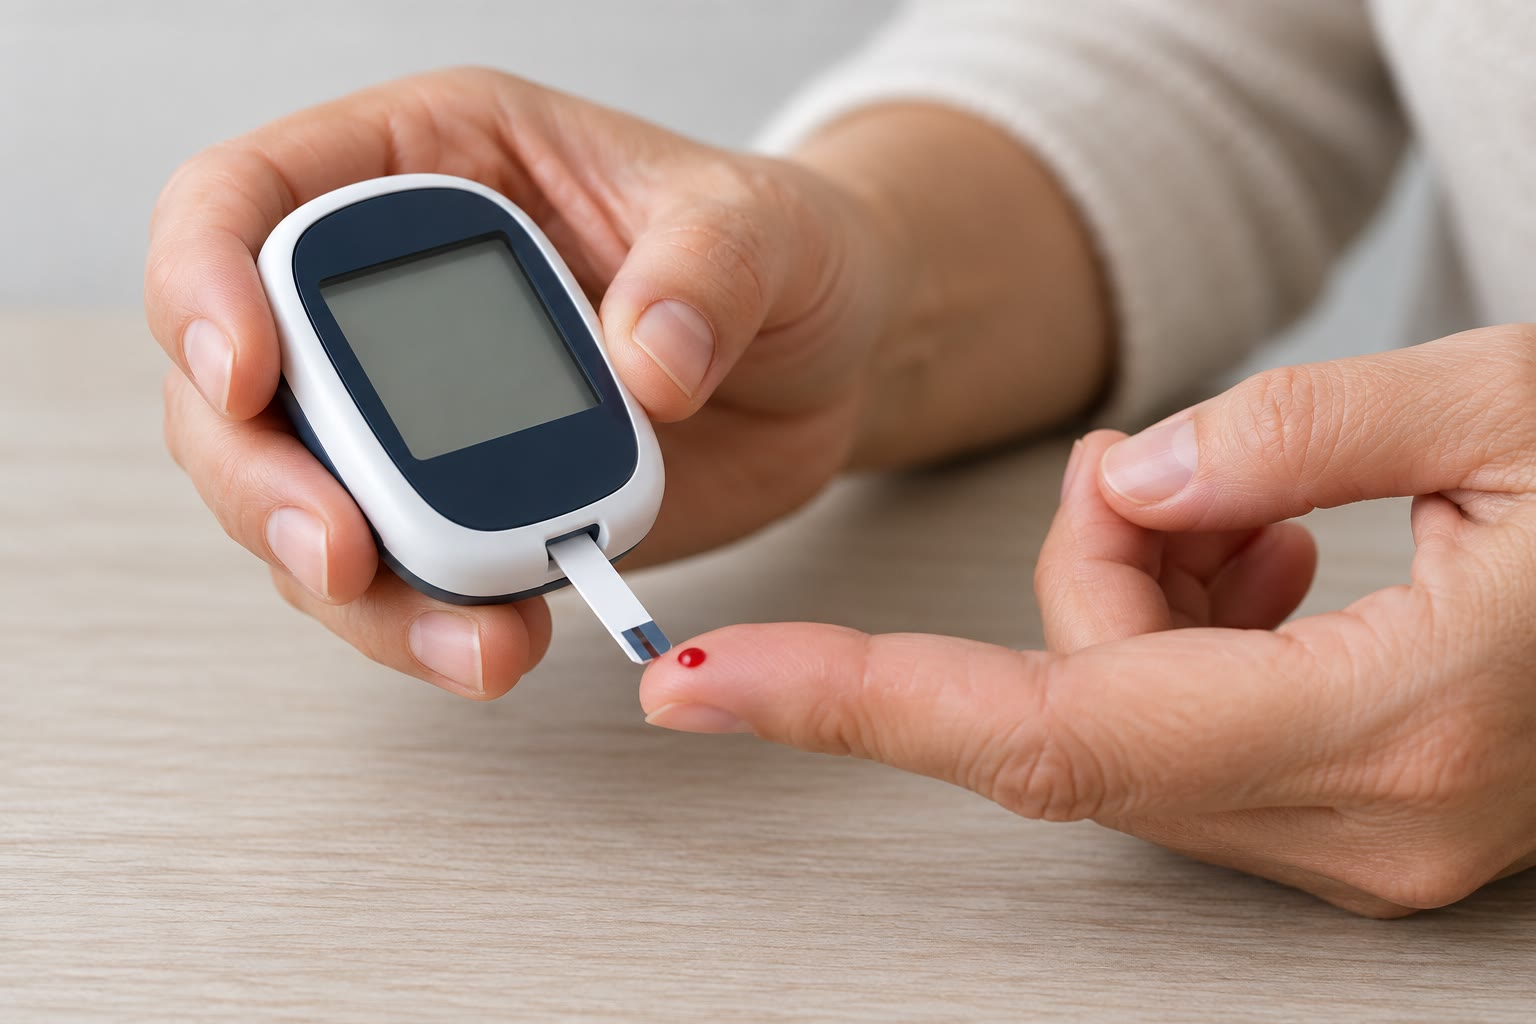
\includegraphics[width=0.6\linewidth]{images/book4/ai/b3-15-glucose-meter.jpg}

{\small Um glicosímetro: a tira traz uma minúscula célula de três eletrodos com
uma \omterm{def:b3:complex-kinetics:enzyme}{enzima} e um mediador redox; o aparelho aplica um potencial e lê uma
corrente.}
\end{omfigure}

\section{A interface eletrodo--solução}

Um metal mergulhado em uma solução de eletrólito carrega uma carga superficial, e
a solução responde com uma carga igual e oposta, feita de um excesso de íons de um
sinal. As duas camadas de carga formam um capacitor de espessura molecular.

\begin{definition}[Dupla camada elétrica]\label{def:b3:electrode-kinetics:double-layer}
A \emph{dupla camada elétrica}\index{dupla camada eletrica@dupla camada elétrica} é o
arranjo de cargas em uma interface eletrodo--solução: a carga do metal e a carga
iônica que a compensa na solução. Sua parte compacta, a \emph{camada de
Helmholtz}\index{camada de Helmholtz}, é a camada de íons e de moléculas de solvente
em contato com a superfície; sua \emph{camada difusa}\index{camada difusa} é a região
além dela, onde a agitação térmica espalha os íons em excesso sobre uma distância
da ordem do \emph{comprimento de Debye}\index{comprimento de Debye} $\kappa^{-1}$. A
\emph{capacitância da dupla camada}\index{capacitancia da dupla camada@capacitância da dupla camada} $C_{\mathrm{dl}}$ é a carga
armazenada por unidade de área e por volt de potencial através da interface.
\end{definition}

\begin{proposition}[Comprimento de Debye]\label{prop:b3:electrode-kinetics:debye-length}
Em uma solução de força iônica $I$ (em \unit{mol.m^{-3}}) e permissividade relativa
$\varepsilon_r$, um pequeno potencial $\varphi_0$ no eletrodo decai na solução como
$\varphi = \varphi_0\eu^{-\kappa x}$, com
\[
  \kappa^{-1} = \sqrt{\frac{\varepsilon_r\varepsilon_0RT}{2F^2I}} .
\]
\end{proposition}

\begin{proof}
A equação de Poisson (da física) relaciona o potencial à densidade de carga:
$\dd^2\varphi/\dd x^2 = -\rho/\varepsilon_r\varepsilon_0$. Cada íon obedece à \omterm{def:b3:partition-functions:boltzmann}{distribuição de Boltzmann} no
potencial: $c_i = c_i^{\circ}\eu^{-z_iF\varphi/RT}$, logo $\rho = F\sum_iz_ic_i^{\circ}\eu^{-z_iF\varphi/RT}$. Para $F\varphi \ll RT$,
$\eu^{-z_iF\varphi/RT} \approx 1 - z_iF\varphi/RT$; os termos de ordem zero se cancelam pela
eletroneutralidade, e $\rho \approx -(F^2/RT)\sum_iz_i^2c_i^{\circ}\,\varphi = -(2F^2I/RT)\varphi$. Logo $\dd^2\varphi/\dd x^2 = \kappa^2\varphi$, cuja
solução que se anula longe é $\varphi_0\eu^{-\kappa x}$.
\end{proof}

\begin{example}[A espessura da dupla camada]\label{ex:b3:electrode-kinetics:debye}
% ledger: eps:H2O.25C, const:eps0, const:F, const:R
Em água a \qty{298.15}{K} ($\varepsilon_r = 78.4$) com \qty{0.10}{mol/L} de um sal 1:1 ($I = \qty{100}{mol.m^{-3}}$),
$\kappa^{-1} = \sqrt{78.4 \times \num{8.854e-12} \times 2479/(2 \times 96\,485^2 \times 100)} = \qty{0.96}{nm}$; a \qty{1.0}{mmol/L},
dez vezes mais. Um \omterm{def:b3:electrode-kinetics:transport}{eletrólito suporte} comprime a \omterm{def:b3:electrode-kinetics:double-layer}{camada difusa} a alguns diâmetros
moleculares.
\end{example}

A \omterm{def:b3:electrode-kinetics:double-layer}{camada difusa} se comporta como um capacitor cujas placas estão separadas por
$\kappa^{-1}$: sua capacitância por unidade de área a baixo potencial é $\varepsilon_r\varepsilon_0\kappa$ (o
resultado de Gouy--Chapman; sua dependência com o potencial é admitida). Em série
com a camada compacta de Helmholtz, ela dá a $C_{\mathrm{dl}}$ medida, da ordem de dezenas
de microfarads por centímetro quadrado (o modelo de Stern). Sempre que o potencial
muda, esse capacitor se carrega: uma varredura a $v$ volts por segundo exige uma
corrente capacitiva $C_{\mathrm{dl}}Av$ que não envolve química e se soma a toda medida voltamétrica.

\begin{omfigure}
\begin{tikzpicture}[font=\small, >=Stealth]
  \fill[black!25] (-1.0,0) rectangle (0,3.2);
  \node[rotate=90] at (-0.5,1.6) {metal};
  \foreach \y in {0.3,0.8,...,2.9}{\node[font=\scriptsize] at (-0.15,\y) {$-$};}
  \foreach \y in {0.35,0.95,1.55,2.15,2.75}{\draw[omDef, fill=omDef!20] (0.3,\y) circle (0.18); \node[font=\scriptsize] at (0.3,\y) {$+$};}
  \draw[black!50, dashed] (0.55,0) -- (0.55,3.2);
  \node[font=\scriptsize, anchor=south, align=center] at (0.45,3.25) {plano de\\ Helmholtz};
  \foreach \x/\y/\s in {1.1/0.6/+, 1.4/2.2/+, 1.9/1.3/+, 2.3/2.7/-, 2.6/0.5/+, 3.1/1.8/+, 3.5/0.9/-, 3.9/2.4/+, 4.4/1.4/-, 4.8/0.4/+, 5.1/2.8/-, 5.4/1.9/+}{
    \draw[black!60, fill=white] (\x,\y) circle (0.15); \node[font=\scriptsize] at (\x,\y) {$\s$};}
  \node[font=\scriptsize, anchor=south] at (3.2,3.25) {camada difusa};
  \draw[->] (0,-2.1) -- (6.0,-2.1) node[anchor=north east] {$x$};
  \draw[->] (0,-2.1) -- (0,-0.3) node[anchor=east] {$|\varphi|$};
  \draw[omThm, thick] (0,-0.5) -- (0.55,-1.0) plot[domain=0.55:5.8, samples=40] (\x,{-2.1+1.1*exp(-(\x-0.55)/1.2)});
  \draw[black!40, dashed] (0.55,-2.1) -- (0.55,-0.4);
  \node[omThm, anchor=south west] at (1.3,-1.6) {$|\varphi(x)|$};
  \draw[<->, black!60] (0.55,-2.5) -- (1.75,-2.5) node[midway, below, font=\scriptsize] {$\sim\kappa^{-1}$};
\end{tikzpicture}

{\small A \omterm{def:b3:electrode-kinetics:double-layer}{dupla camada elétrica} (modelo de Gouy--Chapman--Stern, esquema): um metal
carregado negativamente, uma camada compacta de cátions no plano de Helmholtz e uma
\omterm{def:b3:electrode-kinetics:double-layer}{camada difusa} onde os cátions superam os ânions em número sobre alguns
\omterm{def:b3:electrode-kinetics:double-layer}{comprimentos de Debye}. Embaixo, o valor absoluto do potencial (negativo, como a
carga do metal) cai linearmente através da camada compacta e depois
exponencialmente na \omterm{def:b3:electrode-kinetics:double-layer}{camada difusa}.}
\end{omfigure}

\section{Cinética da transferência de elétrons}

Considere a redução $\mathrm{O} + n\,\mathrm{e}^- \to \mathrm{R}$ em um eletrodo mantido no potencial $E$,
cujo potencial de equilíbrio para a solução global seria $E_{\mathrm{eq}}$. A
sobretensão é $\eta = E - E_{\mathrm{eq}}$.

\begin{definition}[Densidade de corrente de troca, coeficiente de transferência, constante de velocidade padrão]\label{def:b3:electrode-kinetics:exchange}
No equilíbrio, as correntes anódica e catódica são iguais e opostas; seu valor
comum por unidade de área é a \emph{densidade de corrente de troca}\index{densidade de corrente de troca} $j_0$. O
\emph{coeficiente de transferência}\index{coeficiente de transferencia@coeficiente de transferência} $\alpha$ ($0 < \alpha < 1$) é a fração da
energia elétrica $nF\eta$ que abaixa a barreira da reação catódica. A
\emph{constante de velocidade padrão}\index{constante de velocidade padrao@constante de velocidade padrão} $k^\circ$ é o valor
comum das constantes de velocidade catódica e anódica no potencial formal $E^{\circ\prime}$.
\end{definition}

\begin{theorem}[Equação de Butler--Volmer]\label{thm:b3:electrode-kinetics:butler-volmer}
Se as concentrações superficiais são iguais às do seio da solução (sem limitação
pelo transporte de massa), a densidade de corrente na sobretensão $\eta$ é, contando
positivas as correntes anódicas,
\[
  j = j_0\bigl[\eu^{(1 - \alpha)f\eta} - \eu^{-\alpha f\eta}\bigr], \qquad f = \frac{nF}{RT}.
\]
Esta é a \emph{equação de Butler--Volmer}\index{equacao de Butler--Volmer@equação de Butler--Volmer}.
\end{theorem}

\begin{proof}
Pela \omterm{def:b3:rate-theories:tst}{teoria do estado de transição}, as constantes de velocidade catódica e anódica são
$k_{\mathrm c} = A\eu^{-\Delta G_{\mathrm c}^{\ddagger}/RT}$ e $k_{\mathrm a} = A\eu^{-\Delta G_{\mathrm a}^{\ddagger}/RT}$. Variar o potencial do eletrodo de $\delta E$
varia a energia de Gibbs da reação $\mathrm{O} + n\,\mathrm{e}^- \to \mathrm{R}$ de $nF\,\delta E$ (os elétrons
no metal ganham $-nF\,\delta E$ de energia elétrica). Suponha, em primeira ordem, que uma
fração $\alpha$ dessa variação vai para a barreira catódica e o resto para a
anódica: $\Delta G_{\mathrm c}^{\ddagger} \to \Delta G_{\mathrm c}^{\ddagger} + \alpha nF\,\delta E$, $\Delta G_{\mathrm a}^{\ddagger} \to \Delta G_{\mathrm a}^{\ddagger} - (1 - \alpha)nF\,\delta E$. Medir $\delta E$
a partir do potencial de equilíbrio, onde as duas correntes valem ambas $j_0$ em
módulo, dá $j_{\mathrm c} = j_0\eu^{-\alpha f\eta}$ e $j_{\mathrm a} = j_0\eu^{(1 - \alpha)f\eta}$; a corrente líquida é sua
diferença.
\end{proof}

\begin{corollary}[Resistência de transferência de carga]\label{cor:b3:electrode-kinetics:linear}
Para $|\eta| \ll RT/nF$, $j = j_0f\eta$: a interface se comporta como uma resistência
$R_{\mathrm{ct}} = RT/(nFi_0)$, com $i_0 = j_0A$.
\end{corollary}

\begin{proof}
Desenvolva as duas exponenciais em primeira ordem: $j = j_0[(1 - \alpha)f\eta + \alpha f\eta] = j_0f\eta$; então
$\eta/i = 1/(fi_0)$.
\end{proof}

\begin{corollary}[Equação de Tafel]\label{cor:b3:electrode-kinetics:tafel}
Para $\eta \ll -RT/nF$ (uma sobretensão fortemente catódica), o termo anódico é
desprezível e
\[
  \eta = \frac{2.303\,RT}{\alpha nF}\bigl(\log j_0 - \log|j|\bigr):
\]
$\log|j|$ é linear em $\eta$, com uma inclinação de $1/(\text{\qty{118}{mV}})$ por década a \qty{298}{K} para $\alpha = 0.5$, $n =
1$. Esta é a \emph{equação de Tafel}\index{equacao de Tafel@equação de Tafel}.
\end{corollary}

\begin{proof}
$|j| = j_0\eu^{-\alpha f\eta}$, logo $\ln|j| = \ln j_0 - \alpha f\eta$; converta para logaritmos decimais.
\end{proof}

\begin{definition}[Resistência de transferência de carga, inclinação de Tafel]\label{def:b3:electrode-kinetics:charge-transfer}
A \emph{resistência de transferência de carga}\index{resistencia de transferencia de carga@resistência de transferência de carga} de um
eletrodo é $R_{\mathrm{ct}} = (\partial\eta/\partial i)_{\eta = 0}$. A \emph{inclinação de Tafel}\index{inclinacao de Tafel@inclinação de Tafel}
é a variação da sobretensão por década de corrente na região de Tafel,
$2.303\,RT/\alpha nF$.
\end{definition}

\begin{omfigure}
\begin{tikzpicture}
\begin{axis}[name=bv, omcv, width=0.47\linewidth, height=5.4cm, xmin=-300, xmax=300, ymin=-40, ymax=40,
  xlabel={$\eta$ / mV}, ylabel={$j/j_0$},
  legend style={font=\scriptsize, draw=none, at={(0.03,0.97)}, anchor=north west}, legend cell align=left]
\addplot[omDef, thick] table[x=eta_mV, y=a3] {figdata/out/bachelor-3-butler-volmer.dat};
\addplot[black, thick] table[x=eta_mV, y=a5] {figdata/out/bachelor-3-butler-volmer.dat};
\addplot[omThm, thick] table[x=eta_mV, y=a7] {figdata/out/bachelor-3-butler-volmer.dat};
\legend{$\alpha = 0.3$, $\alpha = 0.5$, $\alpha = 0.7$}
\draw[black!30] (axis cs:-300,0) -- (axis cs:300,0) (axis cs:0,-40) -- (axis cs:0,40);
\end{axis}
\begin{axis}[at={(bv.east)}, anchor=west, xshift=1.2cm, omcv, width=0.47\linewidth, height=5.4cm,
  xmin=-300, xmax=300, ymin=-1.5, ymax=4, xlabel={$\eta$ / mV}, ylabel={$\log|j/j_0|$},
  unbounded coords=jump]
\addplot[omDef, thick] table[x=eta_mV, y=l3] {figdata/out/bachelor-3-butler-volmer.dat};
\addplot[black, thick] table[x=eta_mV, y=l5] {figdata/out/bachelor-3-butler-volmer.dat};
\addplot[omThm, thick] table[x=eta_mV, y=l7] {figdata/out/bachelor-3-butler-volmer.dat};
\draw[black!40, dashed] (axis cs:-300,2.54) -- (axis cs:0,0);
\draw[black!50] (axis cs:-200,1.85) -- (axis cs:-120,3.3) node[anchor=south, font=\scriptsize, inner sep=1pt] {inclinação $1/(\qty{118}{mV})$};
\end{axis}
\end{tikzpicture}

{\small A \omterm{thm:b3:electrode-kinetics:butler-volmer}{equação de Butler--Volmer} ($n = 1$, \qty{298}{K}) para três \omterm{def:b3:electrode-kinetics:exchange}{coeficientes
de transferência}. À esquerda: a corrente é linear em $\eta$ perto do equilíbrio (a
\omterm{def:b3:electrode-kinetics:charge-transfer}{resistência de transferência de carga}) e exponencial além; $\alpha$ a torna
assimétrica. À direita: o gráfico de Tafel, cujos ramos retos extrapolam para
$\log|j/j_0| = 0$ em $\eta = 0$; a reta tracejada é a reta de Tafel catódica para $\alpha = 0.5$.}
\end{omfigure}

\begin{method}[Uma análise de Tafel]\label{met:b3:electrode-kinetics:tafel-analysis}
\begin{enumerate}
  \item Registre a corrente estacionária em função de $\eta$ em uma solução agitada,
        bem abaixo da corrente limite (ou corrija o transporte de massa).
  \item Trace $\log|i|$ em função de $\eta$; ajuste o ramo linear além de cerca de \qty{100}{mV}.
  \item A inclinação dá $\alpha$ (ou $1 - \alpha$ no ramo anódico); o intercepto em $\eta = 0$
        dá $\log i_0$.
  \item Verificação: perto de $\eta = 0$, a inclinação de $i$ em função de $\eta$ é $1/R_{\mathrm{ct}} = nFi_0/RT$.
\end{enumerate}
\end{method}

Os sistemas rápidos e lentos do volume do 2.º ano são os dois extremos desse
quadro: um sistema rápido tem $j_0$ grande, e sua curva corrente--potencial sobe
abruptamente no potencial de equilíbrio; um sistema lento precisa de uma grande
sobretensão antes que passe qualquer corrente. A \omterm{def:b3:electrode-kinetics:exchange}{densidade de corrente de troca}
de uma mesma reação varia de muitas ordens de grandeza de um material de
eletrodo para outro: o desprendimento de hidrogênio é rápido sobre platina e
extremamente lento sobre mercúrio.

\section{Transporte de massa}

\begin{definition}[Modos de transporte de massa]\label{def:b3:electrode-kinetics:transport}
As espécies chegam a um eletrodo por \emph{migração}\index{migracao@migração}, o movimento
dos íons no campo elétrico; por difusão, segundo os gradientes de concentração; e por
\emph{convecção}\index{conveccao@convecção}, o movimento da solução como um todo
(agitação, rotação, escoamento). Um \emph{eletrólito suporte}\index{eletrolito suporte@eletrólito suporte}
é um sal inerte adicionado em grande excesso, que transporta quase toda a
corrente através da solução, de modo que a espécie eletroativa só se move por
difusão e convecção.
\end{definition}

\begin{definition}[Cronoamperometria]\label{def:b3:electrode-kinetics:chronoamperometry}
A \emph{cronoamperometria}\index{cronoamperometria} registra a corrente em função do
tempo depois de um degrau do potencial do eletrodo.
\end{definition}

\begin{theorem}[Equação de Cottrell]\label{thm:b3:electrode-kinetics:cottrell}
Depois de um degrau de potencial em $t = 0$ até um valor no qual a espécie eletroativa é
consumida assim que chega a um eletrodo plano de área $A$, em uma solução em
repouso com \omterm{def:b3:electrode-kinetics:transport}{eletrólito suporte}, a corrente é
\[
  i = nFAc^*\sqrt{\frac{D}{\pi t}},
\]
onde $c^*$ é a concentração no seio da solução e $D$ o coeficiente de difusão. Esta é
a \emph{equação de Cottrell}\index{equacao de Cottrell@equação de Cottrell}.
\end{theorem}

\begin{proof}
A concentração obedece à segunda lei de Fick $\partial c/\partial t = D\,\partial^2c/\partial x^2$, com $c(x, 0) = c^*$,
$c(0, t) = 0$ para $t > 0$ e $c \to c^*$ longe. A função $c = c^*\operatorname{erf}(x/2\sqrt{Dt})$, com
$\operatorname{erf}u = \frac{2}{\sqrt\pi}\int_0^u\eu^{-s^2}\dd s$, satisfaz essas condições: $\operatorname{erf}0 = 0$, $\operatorname{erf}u \to 1$ quando $u \to \infty$
(em $t \to 0$ para todo $x > 0$, e longe). Com $u = x/2\sqrt{Dt}$,
$\partial c/\partial t = c^*\frac{2}{\sqrt\pi}\eu^{-u^2}\partial u/\partial t = -c^*\frac{2}{\sqrt\pi}\eu^{-u^2}\frac{u}{2t}$ e $\partial^2c/\partial x^2 = c^*\frac{2}{\sqrt\pi}(-2u)\eu^{-u^2}\frac{1}{4Dt}$: os
dois lados da lei de Fick concordam. A corrente é o fluxo na superfície: $i =
nFAD(\partial c/\partial x)_{x = 0} = nFADc^*\frac{2}{\sqrt\pi}\frac{1}{2\sqrt{Dt}} = nFAc^*\sqrt{D/\pi t}$. (A unicidade da solução é
admitida.)
\end{proof}

\begin{omfigure}
\begin{tikzpicture}
\begin{axis}[name=pr, width=0.47\linewidth, height=5.2cm, xmin=0, xmax=600, ymin=0, ymax=1.08,
  axis lines=left, xlabel={$x$ / \unit{\micro m}}, ylabel={$c/c^*$},
  tick label style={font=\small}, label style={font=\small},
  legend style={font=\scriptsize, draw=none, at={(0.97,0.03)}, anchor=south east}, legend cell align=left]
\addplot[omDef, thick] table[x=x_um, y=t1] {figdata/out/bachelor-3-cottrell-profiles.dat};
\addplot[black!60, thick] table[x=x_um, y=t2] {figdata/out/bachelor-3-cottrell-profiles.dat};
\addplot[omThm, thick] table[x=x_um, y=t3] {figdata/out/bachelor-3-cottrell-profiles.dat};
\addplot[black, thick, dashed] table[x=x_um, y=t4] {figdata/out/bachelor-3-cottrell-profiles.dat};
\legend{\qty{0.1}{s}, \qty{1}{s}, \qty{4}{s}, \qty{16}{s}}
\end{axis}
\begin{axis}[at={(pr.east)}, anchor=west, xshift=1.3cm, width=0.47\linewidth, height=5.2cm,
  xmin=0, xmax=3.3, ymin=0, ymax=40, axis lines=left, xlabel={$t^{-1/2}$ / \unit{s^{-1/2}}},
  ylabel={$i$ / \unit{\micro A}}, tick label style={font=\small}, label style={font=\small}]
\addplot[omDef, very thick] table[x=tm12, y=i_uA] {figdata/out/bachelor-3-cottrell-current.dat};
\end{axis}
\end{tikzpicture}

{\small \omterm{def:b3:electrode-kinetics:chronoamperometry}{Cronoamperometria} (modelo: $D = \qty{1.0e-5}{cm^2.s^{-1}}$, $c^* = \qty{1.0}{mM}$, um disco de \qty{3}{mm}).
À esquerda: a camada de depleção cresce como $\sqrt{Dt}$, cerca de \qty{30}{\micro m} depois de
\qty{0.1}{s} e \qty{350}{\micro m} depois de \qty{16}{s}. À direita: a corrente de Cottrell é
proporcional a $t^{-1/2}$; sua inclinação dá $D$.}
\end{omfigure}

Uma solução agitada ou um eletrodo de disco rotatório mantêm a camada de difusão
com espessura constante $\delta$: a corrente atinge o valor limite estacionário $nFADc^*/\delta$
do volume do 2.º ano. Para um disco rotatório, $\delta$ diminui como o inverso da raiz
quadrada da velocidade de rotação (Levich, admitido), o que torna a corrente limite
proporcional a $\sqrt\omega$.

\section{Voltametria cíclica}

\begin{definition}[Voltametria cíclica]\label{def:b3:electrode-kinetics:cv}
A \emph{voltametria cíclica}\index{voltametria ciclica@voltametria cíclica} varre o potencial de um
eletrodo de trabalho estacionário linearmente com o tempo entre dois limites, ida
e volta, com uma velocidade de varredura $v$, em uma solução em repouso, e registra a
corrente. O gráfico da corrente em função do potencial é o \emph{voltamograma}\index{voltamograma}; cada
onda tem uma \emph{corrente de pico}\index{corrente de pico} $i_{\mathrm p}$ em seu \emph{potencial de pico}\index{potencial de pico}
$E_{\mathrm p}$.
\end{definition}

O pico surge de dois efeitos concorrentes. À medida que o potencial ultrapassa $E^{\circ\prime}$,
a concentração superficial do reagente cai (a equação de Nernst, para um sistema
rápido) e a corrente cresce; mas a camada empobrecida se espessa com o tempo e o
fluxo diminui. Na varredura de volta, o produto, ainda perto do eletrodo, é
convertido de novo.

\begin{definition}[Reversibilidade]\label{def:b3:electrode-kinetics:reversibility}
Com o parâmetro de velocidade adimensional $\Lambda = k^\circ/\sqrt{DnFv/RT}$, que compara a
velocidade da transferência de elétrons com a velocidade de difusão imposta pela
varredura, um par é \emph{eletroquimicamente reversível}\index{sistema eletroquimicamente reversivel@sistema eletroquimicamente reversível}
se $\Lambda > 15$ (suas concentrações superficiais obedecem à equação de Nernst
a todo instante), \emph{quase reversível}\index{sistema quase reversivel@sistema quase reversível} se $15 >
\Lambda > 10^{-2(1 + \alpha)}$, e \emph{eletroquimicamente irreversível}\index{sistema eletroquimicamente irreversivel@sistema eletroquimicamente irreversível}
abaixo disso.
\end{definition}

\begin{remark}
Os sistemas rápidos e lentos do volume do 2.º ano correspondem a essa
classificação, mas com uma diferença: aqui a reversibilidade depende da velocidade
de varredura. O mesmo par pode ser reversível a \qty{10}{mV/s} e \omterm{def:b3:electrode-kinetics:reversibility}{quase reversível} a
\qty{10}{V/s}, pois uma varredura mais rápida deixa menos tempo para a transferência
de elétrons.
\end{remark}

\begin{proposition}[Equação de Randles--Ševčík]\label{prop:b3:electrode-kinetics:randles-sevcik}
Para uma onda reversível em um eletrodo plano a \qty{298}{K},
\[
  i_{\mathrm p} = 0.4463\,nFAc^*\sqrt{\frac{nFvD}{RT}},
\]
de modo que $i_{\mathrm p} \propto \sqrt v$. Esta é a \emph{equação de Randles--Ševčík}\index{equacao de Randles--Sevcik@equação de Randles--Ševčík}.
\end{proposition}

\begin{proof}[Demonstração parcial]
Nas variáveis $\xi = x\sqrt{nFv/(RTD)}$ e $\theta = nFvt/RT$ (a varredura de potencial em unidades de
$RT/nF$), a lei de Fick com a condição de Nernst na superfície não contém outro
parâmetro além do potencial inicial: o fluxo adimensional é uma função universal
$\chi(\theta)$. De volta às unidades físicas, $i = nFAc^*\sqrt{nFvD/RT}\,\chi(\theta)$: toda
corrente, inclusive a de pico, varia como $\sqrt v$. O valor 0.4463 do máximo de
$\chi$ vem de uma solução numérica (admitido; a simulação da figura o reproduz a
0.1\,\%).
\end{proof}

\begin{proposition}[Separação dos picos]\label{prop:b3:electrode-kinetics:delta-ep}
Para uma onda reversível, os picos catódico e anódico ficam cerca de \qty{28.5}{mV}$/n$
de cada lado de $E^{\circ\prime}$ (a \qty{298}{K}, para um potencial de inversão muito além da onda):
$\Delta E_{\mathrm p} \approx 57/n$ mV, independente da velocidade de varredura, e $E_{1/2} = (E_{\mathrm{pc}} + E_{\mathrm{pa}})/2 =
E^{\circ\prime}$ quando as duas espécies têm coeficientes de difusão iguais.
\end{proposition}

\begin{proof}[Demonstração parcial]
Na forma adimensional da demonstração anterior, o pico ocorre em um valor fixo de
$\theta$, isto é, em um potencial fixo em relação a $E^{\circ\prime}$, qualquer que seja $v$; a
simetria da condição de Nernst entre O e R põe o pico anódico em posição
simétrica. O valor numérico é admitido; a simulação dá
$\pm\qty{28.5}{mV}$, $\Delta E_{\mathrm p} = \qty{57.7}{mV}$.
\end{proof}

\begin{omfigure}
\begin{tikzpicture}
\begin{axis}[name=cv, omcv, width=0.62\linewidth, height=6.4cm, xmin=-320, xmax=320, ymin=-30, ymax=22,
  xlabel={$E - E^{\circ\prime}$ / mV}, ylabel={$i$ / \unit{\micro A}},
  legend style={font=\scriptsize, draw=none, fill=white, fill opacity=0.85, text opacity=1,
  at={(0.01,0.99)}, anchor=north west}, legend cell align=left]
\addplot[black!40, thin] table[x=E_mV, y=i_uA] {figdata/out/bachelor-3-cyclic-voltammetry-v25.dat};
\addplot[omDef!60, thin] table[x=E_mV, y=i_uA] {figdata/out/bachelor-3-cyclic-voltammetry-v50.dat};
\addplot[omDef, thick] table[x=E_mV, y=i_uA] {figdata/out/bachelor-3-cyclic-voltammetry-v100.dat};
\addplot[black, thick] table[x=E_mV, y=i_uA] {figdata/out/bachelor-3-cyclic-voltammetry-v200.dat};
\addplot[omThm, thick, dashed] table[x=E_mV, y=i_uA] {figdata/out/bachelor-3-cyclic-voltammetry-quasi.dat};
\legend{\qty{25}{mV/s}, \qty{50}{mV/s}, \qty{100}{mV/s}, \qty{200}{mV/s}, {quase rev., \qty{100}{mV/s}}}
\end{axis}
\begin{axis}[at={(cv.east)}, anchor=west, xshift=1.3cm, width=0.32\linewidth, height=5.0cm,
  xmin=0, xmax=0.5, ymin=0, ymax=30, axis lines=left, xlabel={$\sqrt v$ / \unit{(V/s)^{1/2}}},
  ylabel={$|i_{\mathrm{pc}}|$ / \unit{\micro A}}, tick label style={font=\small}, label style={font=\small}]
\addplot[only marks, mark=*, omDef] table[x=sqrtv, y=ip_uA] {figdata/out/bachelor-3-cyclic-voltammetry-ip.dat};
\addplot[black, domain=0:0.5] {60.06*x};
\end{axis}
\end{tikzpicture}

{\small \omterm{def:b3:electrode-kinetics:cv}{Voltamogramas} cíclicos simulados por diferenças finitas para uma redução
(modelo: \qty{1.0}{mM}, $D = \qty{1.0e-5}{cm^2.s^{-1}}$, disco de \qty{3}{mm}, $n = 1$; corrente anódica
positiva). Ondas reversíveis em quatro velocidades de varredura: os picos ficam a
\qty{57.7}{mV} um do outro, centrados em $E^{\circ\prime}$, e a \omterm{def:b3:electrode-kinetics:cv}{corrente de pico} cresce como
$\sqrt v$ (à direita, a reta é a \omterm{prop:b3:electrode-kinetics:randles-sevcik}{equação de Randles--Ševčík}). Tracejado: um par \omterm{def:b3:electrode-kinetics:reversibility}{quase
reversível} ($k^\circ = \qty{2e-3}{cm.s^{-1}}$) a \qty{100}{mV/s}, com picos separados por
\qty{162}{mV} e mais baixos.}
\end{omfigure}

\begin{method}[Diagnosticar um voltamograma]\label{met:b3:electrode-kinetics:cv-diagnosis}
\begin{enumerate}
  \item Reversível: $\Delta E_{\mathrm p} \approx 57/n$ mV em todas as velocidades de varredura, $|i_{\mathrm{pa}}/i_{\mathrm{pc}}| = 1$, $i_{\mathrm p} \propto \sqrt v$;
        $E_{1/2}$ dá $E^{\circ\prime}$.
  \item \omterm{def:b3:electrode-kinetics:reversibility}{Quase reversível}: $\Delta E_{\mathrm p}$ cresce com a velocidade de varredura; seu valor dá $k^\circ$.
  \item Irreversível: sem pico de volta; o \omterm{def:b3:electrode-kinetics:cv}{potencial de pico} se desloca de $30/\alpha n$ mV por
        década de velocidade de varredura.
  \item Uma etapa química subsequente (mecanismo EC): o pico de volta é menor que o
        de ida nas varreduras lentas e se recupera nas varreduras rápidas, que
        ultrapassam a química.
  \item Espécies adsorvidas: $i_{\mathrm p} \propto v$, e não $\sqrt v$.
\end{enumerate}
\end{method}

Os potenciais em solventes não aquosos, onde os eletrodos de referência derivam, são
referidos a um padrão interno adicionado no fim do experimento: o par
ferrocênio/ferroceno, rápido e bem-comportado na maioria dos solventes orgânicos.

\begin{method}[Montar uma medida com três eletrodos]\label{met:b3:electrode-kinetics:three-electrode}
\begin{enumerate}
  \item Eletrodo de trabalho (carbono vítreo, platina, ouro) recém-polido;
        contraeletrodo (fio de platina) de área maior; eletrodo de referência
        (Ag/AgCl, ou um fio de prata com padrão interno) perto do eletrodo de
        trabalho.
  \item Solução do analito (cerca de 1 mM) com \qty{0.1}{mol/L} de \omterm{def:b3:electrode-kinetics:transport}{eletrólito
        suporte}, desgaseificada com argônio (o oxigênio dissolvido se reduz a
        potenciais moderadamente negativos e acrescentaria suas próprias ondas).
  \item O potenciostato mantém o potencial entre os eletrodos de trabalho e de
        referência e faz passar a corrente entre o eletrodo de trabalho e o
        contraeletrodo; nenhuma corrente passa pelo eletrodo de referência.
\end{enumerate}
\end{method}

\begin{omfigure}
\begin{tikzpicture}[font=\small, >=Stealth]
  \begin{scope}[scale=1.5]
    \pic[transform shape] at (0,0) {beaker={0.7}{omWater!60}};
    \pic[transform shape] at (-0.45,0.35) {electrode={black!70}};
    \pic[transform shape] at (0,0.35) {electrode={black!20}};
    \pic[transform shape] at (0.45,0.35) {probe};
  \end{scope}
  \draw[thick] (-1.6,6.0) rectangle (1.6,7.2);
  \node at (0,6.6) {potenciostato};
  \draw[thick, omDef] (-0.675,4.35) |- (-1.0,5.2) -- (-1.0,6.0);
  \draw[thick, black!60] (0,4.35) -- (0,6.0);
  \draw[thick, omThm] (0.675,5.18) |- (1.0,5.5) -- (1.0,6.0);
  \node[omDef, anchor=east, align=right, font=\scriptsize] at (-1.1,5.2) {trabalho};
  \node[black!70, rotate=90, anchor=north, font=\scriptsize, inner sep=1pt] at (0.06,5.35) {contra};
  \node[omThm, anchor=west, align=left, font=\scriptsize] at (1.1,5.2) {referência};
\end{tikzpicture}

{\small Uma célula de três eletrodos. O potenciostato controla o potencial do
eletrodo de trabalho em relação ao eletrodo de referência, que não conduz
corrente, e impele a corrente através do contraeletrodo.}
\end{omfigure}

\section{Métodos eletroanalíticos}

\begin{definition}[Amperometria, biossensor]\label{def:b3:electrode-kinetics:amperometry}
A \emph{amperometria}\index{amperometria} mede a corrente em um potencial fixo,
proporcional à concentração da espécie que reage. Um
\emph{biossensor}\index{biossensor} acopla um elemento de reconhecimento biológico
(uma \omterm{def:b3:complex-kinetics:enzyme}{enzima}, um anticorpo) a um transdutor, aqui um eletrodo.
\end{definition}

Na tira de glicose, a glicose oxidase oxida a glicose a gliconolactona e é
regenerada por um mediador, o hexacianoferrato(III), que é reduzido; no eletrodo,
mantido em um potencial em que o hexacianoferrato(II) é oxidado, a corrente mede o
mediador formado, dois por glicose:
\[
  \ce{C6H12O6 + 2 [Fe(CN)6]^3- -> C6H10O6 + 2 [Fe(CN)6]^4- + 2 H+} .
\]

\begin{definition}[Voltametria de redissolução anódica]\label{def:b3:electrode-kinetics:stripping}
A \emph{voltametria de redissolução anódica}\index{voltametria de redissolucao anodica@voltametria de redissolução anódica}
pré-concentra um metal reduzindo seus íons sobre um eletrodo durante um tempo fixo,
em um potencial fixo, depois varre o potencial no sentido anódico e mede o pico de
corrente de sua reoxidação, que é proporcional à concentração na solução.
\end{definition}

A pré-concentração torna o método sensível o bastante para traços de chumbo ou de
cádmio na água potável, no nível dos microgramas por litro. Como a sensibilidade
depende da matriz, a calibração é feita na própria amostra, por adições padrão.

\begin{method}[Adições padrão com redissolução]\label{met:b3:electrode-kinetics:standard-addition}
\begin{enumerate}
  \item Registre o pico de redissolução da amostra, e depois após três ou mais
        adições de um padrão, cada uma elevando a concentração de uma quantidade
        conhecida (volumes pequenos, de modo que a diluição seja desprezível ou corrigida).
  \item Ajuste a altura do pico em função da concentração adicionada: uma reta.
  \item Seu intercepto no eixo das concentrações é o oposto da concentração da
        amostra; propague as incertezas-padrão da reta até o resultado.
\end{enumerate}
\end{method}

\begin{omfigure}
\begin{tikzpicture}
\begin{axis}[name=sp, omcv, width=0.47\linewidth, height=5.2cm, xmin=-600, xmax=-300, ymin=0, ymax=2.4,
  xlabel={$E$ / mV}, ylabel={$i$ / \unit{\micro A}}]
\addplot[black, thick] table[x=E_mV, y=s0] {figdata/out/bachelor-3-standard-addition-peaks.dat};
\addplot[omDef!50, thick] table[x=E_mV, y=s1] {figdata/out/bachelor-3-standard-addition-peaks.dat};
\addplot[omDef!80, thick] table[x=E_mV, y=s2] {figdata/out/bachelor-3-standard-addition-peaks.dat};
\addplot[omDef, thick] table[x=E_mV, y=s3] {figdata/out/bachelor-3-standard-addition-peaks.dat};
\end{axis}
\begin{axis}[at={(sp.east)}, anchor=west, xshift=1.3cm, width=0.47\linewidth, height=5.2cm,
  xmin=-6, xmax=16, ymin=0, ymax=2.3, axis x line=middle, axis y line=left,
  xlabel={Pb adicionado / \unit{\micro g.L^{-1}}}, ylabel={altura do pico / \unit{\micro A}},
  tick label style={font=\small}, label style={font=\small},
  xlabel style={at={(0.5,-0.18)}, anchor=north}]
\addplot[black, thin] table[x=added, y=h] {figdata/out/bachelor-3-standard-addition-line.dat};
\addplot[only marks, mark=*, omDef] table[x=added, y=h] {figdata/out/bachelor-3-standard-addition-points.dat};
\node[font=\scriptsize, anchor=south] at (axis cs:-4.26,0.05) {$-c_0$};
\end{axis}
\end{tikzpicture}

{\small Redissolução anódica do chumbo com três adições padrão (dados do
\cref{exo:b3:electrode-kinetics:9}). À esquerda: os picos de redissolução crescem
a cada adição. À direita: a reta de mínimos quadrados da altura do pico em função
da concentração adicionada corta o eixo no oposto da concentração da amostra.}
\end{omfigure}

\begin{definition}[Eletrodo íon-seletivo, coeficiente de seletividade]\label{def:b3:electrode-kinetics:ise}
Um \emph{eletrodo íon-seletivo}\index{eletrodo ion-seletivo@eletrodo íon-seletivo} é um eletrodo
cujo potencial, por meio de uma membrana que troca preferencialmente um íon,
depende da atividade desse íon. Seu \emph{coeficiente de
seletividade}\index{coeficiente de seletividade} $K_{ij}$ mede sua resposta a um íon
interferente $j$ em relação ao íon principal $i$.
\end{definition}

\begin{proposition}[Equação de Nikolsky]\label{prop:b3:electrode-kinetics:nikolsky}
Para um íon principal $i$ de carga $z_i$ e um íon interferente $j$ de carga $z_j$,
\[
  E = \text{const} + \frac{RT}{z_iF}\ln\bigl(a_i + K_{ij}a_j^{z_i/z_j}\bigr) .
\]
Esta é a \emph{equação de Nikolsky}\index{equacao de Nikolsky@equação de Nikolsky}.
\end{proposition}

\begin{proof}[Demonstração parcial]
Para uma membrana permeável apenas a $i$, a igualdade dos potenciais eletroquímicos
através dela dá um potencial do tipo de Nernst, $\frac{RT}{z_iF}\ln a_i$ mais uma constante.
Se $j$ pode substituir $i$ na membrana por troca iônica, com uma constante de troca
que define $K_{ij}$, a atividade de $i$ na superfície da membrana é aumentada de
$K_{ij}a_j^{z_i/z_j}$ (a potência mantém as cargas equilibradas na troca). A dedução
detalhada é admitida.
\end{proof}

O eletrodo de vidro de pH é o mais antigo \omterm{def:b3:electrode-kinetics:ise}{eletrodo íon-seletivo}; seu erro de sódio,
em pH alto e concentração alta de sódio, é o termo de Nikolsky.

\begin{definition}[Coulometria]\label{def:b3:electrode-kinetics:coulometry}
A \emph{coulometria}\index{coulometria} determina a quantidade de uma substância a partir
da carga total que passa em sua eletrólise completa: $Q = nFn_{\text{substância}}$ (lei de
Faraday), sem nenhuma calibração.
\end{definition}

\begin{proposition}[Incerteza de uma concentração lida em uma reta de calibração]\label{prop:b3:electrode-kinetics:inverse-prediction}
Para uma reta de calibração $y = a + bx$ ajustada a $n$ padrões (desvio-padrão
residual $s$, média $\bar y$, $S_{xx} = \sum(x_i - \bar x)^2$), a concentração de uma amostra cuja
resposta média sobre $m$ réplicas é $y_0$ vale $x_0 = (y_0 - a)/b$, com a incerteza-padrão
\[
  u(x_0) = \frac{s}{b}\sqrt{\frac1m + \frac1n + \frac{(y_0 - \bar y)^2}{b^2S_{xx}}} .
\]
\end{proposition}

\begin{proof}
Escreva $x_0 = \bar x + (y_0 - \bar y)/b$. Em primeira ordem, sua variância é $(\operatorname{var}y_0 +
\operatorname{var}\bar y)/b^2 + (y_0 - \bar y)^2\operatorname{var}b/b^4$, sendo os três termos não correlacionados ($\bar y$ e $b$
não são correlacionados, \cref{prop:b3:rate-theories:slope-uncertainty}). Com $\operatorname{var}y_0 =
s^2/m$, $\operatorname{var}\bar y = s^2/n$ e $\operatorname{var}b = s^2/S_{xx}$, o resultado decorre.
\end{proof}

A incerteza é mínima no meio da faixa de calibração e cresce em direção às suas
extremidades; leituras repetidas da amostra reduzem apenas o primeiro termo.

\begin{inthelab}[Preparar um eletrodo de carbono vítreo]
O eletrodo é polido sobre um feltro com uma suspensão de alumina, em movimentos
em forma de oito, enxaguado, colocado brevemente em ultrassom na água e enxaguado
de novo. Um \omterm{def:b3:electrode-kinetics:cv}{voltamograma} de um par conhecido (hexacianoferrato, ferroceno) verifica
que a separação dos picos está próxima do valor reversível: uma separação maior
indica uma superfície suja ou uma resistência não compensada. A solução é
desgaseificada com argônio durante dez minutos e mantida sob uma camada de
argônio durante as varreduras.
\end{inthelab}

\begin{safety}{\ghs[0.62cm]{GHS03}\ghs[0.62cm]{GHS05}\ghs[0.62cm]{GHS07}\ghs[0.62cm]{GHS08}\ghs[0.62cm]{GHS09}}
% ledger: ghs4:PbNO32, ghs4:K3FeCN6
Nitrato de chumbo, usado para os padrões de chumbo: oxidante, pode prejudicar a
fertilidade e o feto, suspeito de ser cancerígeno, muito tóxico para os organismos
aquáticos; as soluções padrão são compradas prontas e manipuladas com luvas, e todo
resíduo de chumbo é recolhido. Hexacianoferrato(III) de potássio: nocivo e suspeito
de prejudicar a fertilidade; nunca fortemente acidificado nem aquecido (poderia
liberar cianeto de hidrogênio). Os eletrodos de mercúrio, antes comuns na análise
por redissolução, foram substituídos por eletrodos de filme de bismuto e de carbono.
\end{safety}

\begin{history}[O polarógrafo de Heyrovský, 1922]
Jaroslav Heyrovský mediu em 1922 a corrente através de um eletrodo de mercúrio que
gotejava de um capilar fino, renovando sua superfície a cada poucos segundos, em
função do potencial aplicado. Cada espécie redutível dava uma onda cuja posição a
identificava e cuja altura media sua concentração; com Masuzo Shikata, ele
construiu em 1924 o polarógrafo, que registrava as curvas automaticamente em papel
fotográfico. A polarografia foi o primeiro método instrumental de análise química
de uso rotineiro e valeu a Heyrovský o Prêmio Nobel de Química de 1959.
\end{history}

\section{Exercícios}

\begin{exercise}[$\star$]\label{exo:b3:electrode-kinetics:1}
Um gráfico de Tafel de uma redução ($n = 1$, \qty{298}{K}) tem inclinação catódica de $-\qty{118}{mV}$
por década e extrapola em $\eta = 0$ para $|j| = \qty{2.0e-6}{A.cm^{-2}}$ (dados do exercício).
Dê $\alpha$ e $j_0$.
\end{exercise}

\begin{exercise}[$\star$]\label{exo:b3:electrode-kinetics:2}
Um eletrodo de \qty{0.20}{cm^2} tem $j_0 = \qty{1.0e-3}{A.cm^{-2}}$ para um par de um elétron.
Calcule sua \omterm{def:b3:electrode-kinetics:charge-transfer}{resistência de transferência de carga} a \qty{298}{K}.
\end{exercise}

\begin{exercise}[$\star$]\label{exo:b3:electrode-kinetics:3}
% ledger: eps:H2O.25C
Calcule o \omterm{def:b3:electrode-kinetics:double-layer}{comprimento de Debye} em água a \qty{298.15}{K} para \qty{1.0}{mmol/L} e para \qty{0.10}{mol/L}
de \ce{MgSO4}.
\end{exercise}

\begin{exercise}[$\star$]\label{exo:b3:electrode-kinetics:4}
Um \omterm{def:b3:electrode-kinetics:cv}{voltamograma} cíclico a \qty{100}{mV/s} em um eletrodo de \qty{0.0707}{cm^2} com $C_{\mathrm{dl}} =
\qty{20}{\micro F.cm^{-2}}$: calcule a corrente capacitiva e compare com o pico faradaico de
\qty{19}{\micro A} da figura. O que acontece a \qty{10}{V/s}?
\end{exercise}

\begin{exercise}[$\star\star$]\label{exo:b3:electrode-kinetics:5}
Depois de um degrau de potencial, $i\sqrt t = \qty{12.2}{\micro A.s^{1/2}}$ para a redução a um elétron de uma
solução \qty{1.00}{mM} em um eletrodo de \qty{0.0707}{cm^2}. Calcule $D$.
\end{exercise}

\begin{exercise}[$\star\star$]\label{exo:b3:electrode-kinetics:6}
Calcule a \omterm{def:b3:electrode-kinetics:cv}{corrente de pico} de Randles--Ševčík para $n = 1$, $A = \qty{0.0707}{cm^2}$, $c^* = \qty{2.0}{mM}$,
$D = \qty{7.0e-6}{cm^2.s^{-1}}$ a \qty{50}{mV/s} e a \qty{500}{mV/s}.
\end{exercise}

\begin{exercise}[$\star\star$]\label{exo:b3:electrode-kinetics:7}
Três pares dão, a 50 e a \qty{500}{mV/s}: (a) $\Delta E_{\mathrm p} = 58$ e 59 mV, $|i_{\mathrm{pa}}/i_{\mathrm{pc}}| = 1.0$;
(b) $\Delta E_{\mathrm p} = 75$ e 140 mV, $|i_{\mathrm{pa}}/i_{\mathrm{pc}}| = 1.0$; (c) $\Delta E_{\mathrm p}$ indefinido a \qty{50}{mV/s} (sem
pico de volta), um pico de volta com $|i_{\mathrm{pa}}/i_{\mathrm{pc}}| = 0.8$ a \qty{500}{mV/s}. Diagnostique cada um.
\end{exercise}

\begin{exercise}[$\star\star$]\label{exo:b3:electrode-kinetics:8}
Um eletrodo seletivo ao potássio tem $K_{\ce{K+},\ce{Na+}} = \num{2e-4}$. Em uma amostra com $a(\ce{K+}) =
\qty{4.0e-3}{}$ e $a(\ce{Na+}) = 0.14$, qual é o erro relativo sobre a atividade do potássio se o
sódio for ignorado?
\end{exercise}

\begin{exercise}[$\star\star$]\label{exo:b3:electrode-kinetics:9}
Os picos de redissolução de uma amostra de água com 0, 5, 10 e \qty{15}{\micro g.L^{-1}} de chumbo
adicionado valem 0.468, 1.003, 1.571 e \qty{2.101}{\micro A} (dados do exercício). Calcule a
concentração de chumbo da solução medida, com sua incerteza-padrão.
\end{exercise}

\begin{exercise}[$\star\star\star$]\label{exo:b3:electrode-kinetics:10}
Um coulômetro de cobre faz passar uma corrente constante de \qty{50.0}{mA} durante \qty{30.0}{min} e deposita
cobre a partir de \ce{Cu^{2+}}. Calcule a massa depositada; por que a \omterm{def:b3:electrode-kinetics:coulometry}{coulometria} não
precisa de calibração?
\end{exercise}

\begin{exercise}[$\star\star\star$]\label{exo:b3:electrode-kinetics:11}
Para um par com $k^\circ = \qty{1.0e-2}{cm.s^{-1}}$ e $D = \qty{1.0e-5}{cm^2.s^{-1}}$, calcule $\Lambda$ a \qty{0.1}{V/s}
e a \qty{10}{V/s} ($n = 1$, \qty{298}{K}) e classifique a onda em cada velocidade de varredura.
\end{exercise}

\begin{exercise}[$\star\star\star$]\label{exo:b3:electrode-kinetics:12}
Uma reta de calibração obtida com $n = 7$ padrões tem $b = \qty{0.919}{\micro A.mM^{-1}}$, $s = \qty{0.077}{\micro A}$,
$\bar y = \qty{8.89}{\micro A}$ e $S_{xx} = \qty{241}{mM^2}$. Calcule a incerteza de uma concentração lida
a partir de uma leitura em $y_0 = \bar y$ e em $y_0 = \qty{18.0}{\micro A}$, e a partir de três leituras em $\bar y$.
\end{exercise}

\section{Problema: A tira de glicose}

\begin{problem}[{Problema de fim de semana --- a tira de glicose: a enzima e seu
mediador, a cronoamperometria e o coeficiente de difusão, a reta de calibração e uma
amostra de sangue com sua incerteza, e a interferência do ascorbato}]
\label{pb:b3:electrode-kinetics:1}
% ledger: const:F
Uma tira de teste traz glicose oxidase, hexacianoferrato(III) de potássio e um
eletrodo de trabalho de carbono de \qty{0.0300}{cm^2}. Dados do problema: (a) uma tira
cheia de hexacianoferrato(II) \qty{10.0}{mM} e submetida a um degrau até um potencial
oxidante dá as correntes 42.0, 29.3, 24.1, 20.8 e \qty{18.7}{\micro A} em 1, 2, 3, 4 e \qty{5}{s};
(b) padrões de glicose de 2.0, 4.0, 6.0, 8.0, 10.0, 15.0 e \qty{20.0}{mM} dão, em
\qty{5.0}{s}, 2.16, 4.08, 5.83, 7.78, 9.45, 14.23 e \qty{18.69}{\micro A}; (c) uma amostra de sangue dá
\qty{7.10}{\micro A}.

\medskip\noindent\textbf{Parte I --- A química.}
\begin{enumerate}
  \item Escreva as semirreações da glicose (até a gliconolactona, \ce{C6H10O6}) e do
        mediador, e a reação global balanceada.
  \item Quantos elétrons chegam ao eletrodo por molécula de glicose?
  \item Por que se usa um mediador em vez do oxigênio, o parceiro natural da
        \omterm{def:b3:complex-kinetics:enzyme}{enzima}?
  \item Por que o eletrodo é mantido em um potencial em que o hexacianoferrato(II)
        é oxidado, bem além de seu potencial formal?
  \item Por que a leitura precisa ser feita em um tempo fixo depois da aplicação
        da gota?
\end{enumerate}

\medskip\noindent\textbf{Parte II --- \omterm{def:b3:electrode-kinetics:chronoamperometry}{Cronoamperometria}.}
\begin{enumerate}[resume]
  \item Que lei as correntes de (a) devem seguir? Verifique-a nos dados.
  \item Ajuste $i$ em função de $t^{-1/2}$ passando pela origem: a inclinação é \qty{41.8}{\micro A.s^{1/2}}. Deduza
        o $D$ do hexacianoferrato(II).
  \item Calcule a espessura $\sqrt{\pi Dt}$ da camada de depleção depois de \qty{5}{s}. O
        modelo plano é razoável para uma tira cuja camada de solução tem cerca de
        \qty{100}{\micro m} de espessura?
  \item Qual seria a corrente em \qty{5}{s} com \qty{5.0}{mM} em vez de \qty{10.0}{mM}?
\end{enumerate}

\medskip\noindent\textbf{Parte III --- Calibração.}
\begin{enumerate}[resume]
  \item A reta de mínimos quadrados de (b) tem $a = \qty{0.356}{\micro A}$ ($s_a = 0.054$), $b =
        \qty{0.9189}{\micro A.mM^{-1}}$ ($s_b = 0.0049$), $s = \qty{0.077}{\micro A}$. O que $a$ representa?
  \item A resposta é linear em toda a faixa? O que a limitaria em concentrações altas
        de glicose?
  \item Calcule a concentração de glicose da amostra de sangue.
  \item Com $\bar y = \qty{8.89}{\micro A}$ e $S_{xx} = \qty{241}{mM^2}$, calcule sua incerteza-padrão.
  \item Que termo da incerteza domina, e como ele poderia ser reduzido?
  \item Estime o limite de detecção como $3s/b$.
  \item Exprima o resultado em miligramas por decilitro (massa molar da glicose
        \qty{180.16}{g/mol}).
\end{enumerate}

\medskip\noindent\textbf{Parte IV --- Interferentes.}
\begin{enumerate}[resume]
  \item O ascorbato (vitamina C) é oxidado diretamente no eletrodo. O que ele faz
        com a leitura?
  \item Como um \omterm{def:b3:electrode-kinetics:cv}{voltamograma} cíclico da tira o revelaria?
  \item Por que um potencial de trabalho mais baixo, possibilitado por um mediador
        melhor, reduz essas interferências?
  \item Um eletrodo branco sem \omterm{def:b3:complex-kinetics:enzyme}{enzima}, lido no mesmo instante, dá \qty{0.25}{\micro A}
        a mais que o intercepto da calibração com uma dada amostra. Como ele é usado?
  \item Como a temperatura da tira afeta a corrente, por meio de $D$?
  \item Por que os padrões são preparados em uma matriz semelhante ao sangue?
  \item Por que a incerteza do aparelho é, na prática, maior que a calculada na
        Parte III?
  \item Enuncie o resultado: a concentração de glicose da amostra, com sua
        incerteza-padrão.
\end{enumerate}
\end{problem}
